\documentclass[12pt]{article}%
\usepackage{amsfonts}
\usepackage{hyperref}
\usepackage{fancyhdr}
\usepackage{comment}
\usepackage{mathrsfs}
\usepackage{mathtools}
\usepackage{graphicx}
\usepackage[a4paper, top=2.5cm, bottom=2.5cm, left=2.2cm, right=2.2cm]%
{geometry}
\usepackage{times}
\usepackage{amsmath}
\usepackage{amsthm}
%\usepackage{changepage}
\usepackage{amssymb}
%\usepackage{graphicx}%
\setcounter{MaxMatrixCols}{30}
\newtheorem{theorem}{Theorem}
\newtheorem{acknowledgement}[theorem]{Acknowledgement}
\newtheorem{algorithm}[theorem]{Algorithm}
\newtheorem{axiom}{Axiom}
\newtheorem{case}[theorem]{Case}
\newtheorem{claim}[theorem]{Claim}
\newtheorem{conclusion}[theorem]{Conclusion}
\newtheorem{condition}[theorem]{Condition}
\newtheorem{conjecture}[theorem]{Conjecture}
\newtheorem{corollary}[theorem]{Corollary}
\newtheorem{criterion}[theorem]{Criterion}
\newtheorem{definition}[theorem]{Definition}
\newtheorem{example}[theorem]{Example}
\newtheorem{exercise}[theorem]{Exercise}
\newtheorem{lemma}[theorem]{Lemma}
\newtheorem{notation}[theorem]{Notation}
\newtheorem{problem}[theorem]{Problem}
\newtheorem{proposition}[theorem]{Proposition}
\newtheorem{remark}[theorem]{Remark}
\newtheorem{solution}[theorem]{Solution}
\newtheorem{summary}[theorem]{Summary}

\newcommand{\Q}{\mathbb{Q}}
\newcommand{\R}{\mathbb{R}}
\newcommand{\C}{\mathbb{C}}
\newcommand{\Z}{\mathbb{Z}}

\newcommand{\E}{\mathrm{E}}
\newcommand{\Var}{\mathrm{Var}}
\newcommand{\Cov}{\mathrm{Cov}}

\begin{document}

\title{MATH618 Homework 4}
\author{Fernando}
\date{\today}
\maketitle
\section*{Problem 1}
\subsection*{Question 1}
We want to find $u$ such that:
\[
	\mathcal{L}u=\lambda u
\]
so
\[
	(\mathcal{L}-\lambda I) u=0
\]
We know that under this conditions $\sin(n\pi x)$ forms a basis so if we
identify $u$ with its sequence of Fourier coefficients we get
\begin{align*}
	(\mathcal{L}-\lambda I)\{U_n\}=0\\
	\left\{\frac{U_n}{n^2\pi^2}-\lambda U_n\right\}=0\\
	\left\{U_n\left(\frac{1}{n^2\pi^2}-\lambda\right)\right\}=0
\end{align*}
then for each $n$ $U_n=0$ or $\lambda=\frac{1}{n^2\pi^2}$. If $U_n=0$ for all
$n$ then we get the trivial solution which we are not interested in. Then
$\lambda = \frac{1}{n^2 \pi^2}$ but since $\lambda$ can not change that means
that $U_n=0$ for all $n$ except one.

\textbf{Conclusion:} The eigenvalues are $\lambda_n=\frac{1}{n^2\pi^2}$ and the
associated sequences are the $e_n$ (standard basis). Going back to the space of
functions we get that the eigenfunctions are
\[
	\sin(n\pi x)
\]
and they are associated to the same eigenvalues, i.e.
$\lambda_n=\frac{1}{n^2\pi^2}$.
\subsection*{Question 2}
The eigenvalues of $\mathcal{L}$ are $\lambda_n=\frac{1}{n^2\pi^2}$.
\subsection*{Question 3}
The eigenvalues go to zero.
\subsection*{Question 4}
\subsection*{Question 5}
\section*{Problem 2}
\section*{Problem 3}
\subsection*{Question 1}
We start with a bounded set $A$ and consider its image under the
identity operator i.e. $A$ again. Since $A$ is bounded $\overline{A}$ is
bounded and closed, and because we are in a finite dimensional space, this is
equivalent to compact.
\subsection*{Question 2}
Consider the unit ball, we know it is bounded. Its image under the identity map
is itself, so its closure is the closed unit ball, which is not compact.
\section*{Problem 4}
Here is my current understanding of the problem.

We were trying to show that $l_\infty$ is not separable. \textbf{What does that mean?}

It means that there is no countable basis whose closure spans the
entire space.

\textbf{Now the question is what do we mean by span?}

We mean all \textbf{finite} linear combinations.

\textbf{Why not infinite?}

This question is answered at the end of the problem.

\textbf{So for now lets work with finite linear combinations.}

Now we proceed as described in the homework.

\textbf{Step 1:} Pretend we had a countable set $\{x_i\}_{i=1}^\infty$ whose
closure spans $l_\infty$.

\textbf{Step 2:} We define
\[
	S_\mathbb{Q}\coloneqq\left\{ y\in l_\infty : \exists N \in \mathbb{N}:
	y=\sum_{i=1}^N \alpha_ix_i, \alpha_i \in \mathbb{Q}\right\},
\]
which is basically the rational span of $\{x_i\}$, and show that it is
countable.

\textbf{Steps 3 and 4:} Notice that in any $\varepsilon$-neighborhood of $x\in
l_\infty$ there needs to be a point of $S_\mathbb{Q}$.

\textbf{Step 5:} Since there are uncountably many elements that are one unit
apart in $l_\infty$ then $S_\mathbb{Q}$ has uncountably many elements (a
contradiction!!). Which concludes of the proof. $\qedsymbol$

Let's show \textbf{Step 2}, i.e. $S_\mathbb{Q}$ is countable. In order to do this we must
create an injective map from $S_\mathbb{Q}$ to $\mathbb{N}$. First observe
that because $\mathbb{Q}$ is countable there exists $f:\mathbb{Q}\to\mathbb{N}$
injective. Now let $P_i$ denote the $i$-th prime number. Then one possible
mapping we can use for this problem is
\[
	\sum_i^N \alpha_ix_i \mapsto \prod_i^N p_i^{f(\alpha_i)}.
\]
Notice that this is well defined and also injective because if $x\neq y$ then
they differ in at least one of the $\alpha_i$'s, which implies they will be
mapped to different numbers by the fundamental theorem of arithmetic (the prime
factorization of natural numbers is unique). Which concludes the proof. \qedsymbol

\textbf{What about infinite linear combinations?}

For all I could find online when we say separable space it is using the
definition of finite linear combinations (Hamel basis).
What if we allowed infinite sums in our definition of span, this is basically
saying that we want to find a Schauder basis instead of a Hamel basis. There
are multiple problems with this. Firstly the sum might not be well defined at
all, secondly and perhaps most importantly $l_\infty$ doesn't have a Schauder
basis! In fact any space with a Schauder basis is separable according to a
proof I found \underline{\href{https://math.stackexchange.com/questions/297851/how-to-prove-that-if-a-normed-space-has-schauder-basis-then-it-is-separable-wh}{here}}.
\section*{Problem 5}
\subsection*{Part a}
Consider $x=(1,-1,1,-1,\dots)$ and $y=(1,1,1,1,\dots)$, then
\[
	\langle x,y \rangle=\sum_ix_iy_i
\]
is not defined because the sum is not convergent.
\subsection*{Part b}
In this case the problem is that $X$ is not complete with respect
to the norm given, and this is a requirement for $X$ to be a
Hilbert space. As to why $X$ is not complete consider the sequence
of functions
\[
	f_n(x)=\begin{cases}
		x=0 \quad x\leq0.5-\frac{1}{n+2}\\
		x=0.5(n+2)(x-(0.5-\frac{1}{n+2})) \quad 0.5-\frac{1}{n+2}\leq x \leq 0.5 +\frac{1}{n+2}\\
		x=1 \quad 0.5 +\frac{1}{n+2} \leq x
		\end{cases}
\]
They look like:

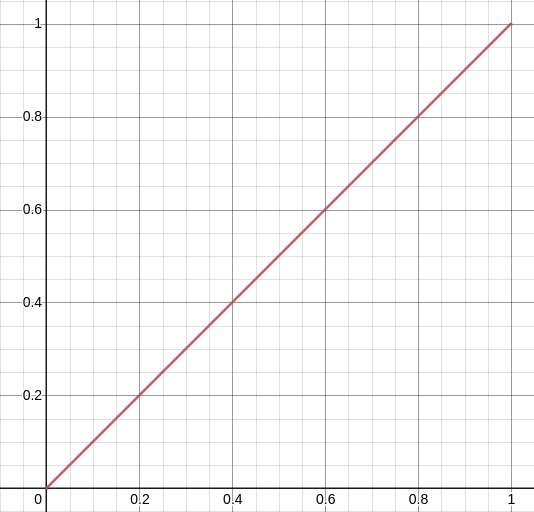
\includegraphics[width=0.3\textwidth]{f1.png}
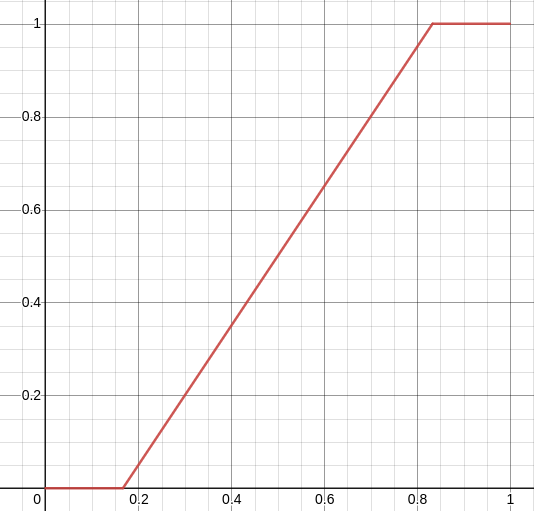
\includegraphics[width=0.3\textwidth]{f2.png}
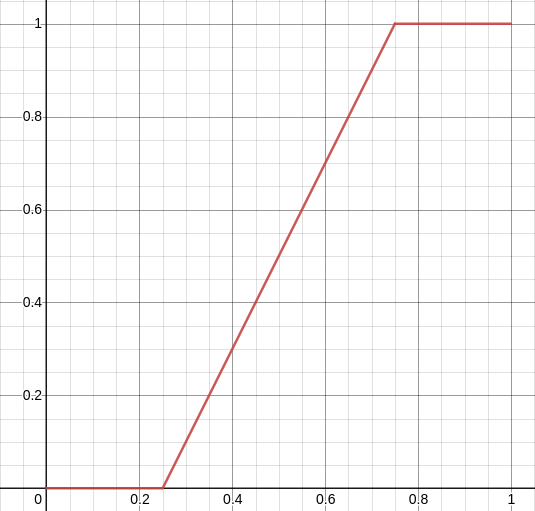
\includegraphics[width=0.3\textwidth]{f3.png}

We know that this sequence converges in $L_2$ to a step function. Which is not
continuous.
\subsection*{Part c}
The problem here is that for this space some functions are not bounded, for
example $\log(x)\in X$ because $\int_0^1\log^2=2<\infty$ but it has infinite
norm. And notice that it is unbounded in a non-trivial way, so if we replace
sup by esssup it is still unbounded. Now we could think of throwing away the
element with infinite norm but then we would end up with $L_\infty$ so it's no
longer the $X$ we started with.
\section*{Problem 6}
I would like to make a presentation on the paper: "Can you hear the shape of a
drum?" If possible I would like to cover the following points
\begin{itemize}
\item	Physical explanation of the problem
\item	Mathematical formulation of the problem
\item	Examples on how different domains sound
\item	Answer to the problem
\item	Discrete analogues
\end{itemize}
The last one is the least related to the course because it is basically linear
algebra but I still think is very interesting and it goes back to the recurrent
theme we have seen in class that in infinite dimensional spaces some properties
hold but a lot of properties don't, so I think it is worth doing the comparison.

\nocite{Schauder_then_separable}
\bibliographystyle{plain}
\bibliography{bibl}
\end{document}
